%%%%%%%%%%%%%%%%%%%%%%%%%%%%%%%%%%%%%%%%%
% Beamer Presentation
% LaTeX Template
% Version 1.0 (10/11/12)
%
% This template has been downloaded from:
% http://www.LaTeXTemplates.com
%
% License:
% CC BY-NC-SA 3.0 (http://creativecommons.org/licenses/by-nc-sa/3.0/)
%
%%%%%%%%%%%%%%%%%%%%%%%%%%%%%%%%%%%%%%%%%

%----------------------------------------------------------------------------------------
%	PACKAGES AND THEMES
%----------------------------------------------------------------------------------------

\documentclass{beamer}

\mode<presentation> {
	\usepackage[utf8]{vietnam}
	\newcommand\tab[1][1cm]{\hspace*{#1}}
	\graphicspath{ {images/} }
	% The Beamer class comes with a number of default slide themes
	% which change the colors and layouts of slides. Below this is a list
	% of all the themes, uncomment each in turn to see what they look like.
	
	%\usetheme{default}
	%\usetheme{AnnArbor}
	%\usetheme{Antibes}
	%\usetheme{Bergen}
	%\usetheme{Berkeley}
	%\usetheme{Berlin}
	%\usetheme{Boadilla}
	%\usetheme{CambridgeUS}
	%\usetheme{Copenhagen}
	%\usetheme{Darmstadt}
	%\usetheme{Dresden}
	%\usetheme{Frankfurt}
	%\usetheme{Goettingen}
	%\usetheme{Hannover}
	%\usetheme{Ilmenau}
	%\usetheme{JuanLesPins}
	%\usetheme{Luebeck}
	\usetheme[secheader]{Madrid}
	%\usetheme{Malmoe}
	%\usetheme{Marburg}
	%\usetheme{Montpellier}
	%\usetheme{PaloAlto}
	%\usetheme{Pittsburgh}
	%\usetheme{Rochester}
	%\usetheme{Singapore}
	%\usetheme{Szeged}
	%\usetheme{Warsaw}
	
	% As well as themes, the Beamer class has a number of color themes
	% for any slide theme. Uncomment each of these in turn to see how it
	% changes the colors of your current slide theme.
	
	%\usecolortheme{albatross}
	%\usecolortheme{beaver}
	%\usecolortheme{beetle}
	%\usecolortheme{crane}
	%\usecolortheme{dolphin}
	%\usecolortheme{dove}
	%\usecolortheme{fly}
	%\usecolortheme{lily}
	%\usecolortheme{orchid}
	%\usecolortheme{rose}
	%\usecolortheme{seagull}
	%\usecolortheme{seahorse}
	%\usecolortheme{whale}
	%\usecolortheme{wolverine}
	
	%\setbeamertemplate{footline} % To remove the footer line in all slides uncomment this line
	%\setbeamertemplate{footline}[page number] % To replace the footer line in all slides with a simple slide count uncomment this line
	
	%\setbeamertemplate{navigation symbols}{} % To remove the navigation symbols from the bottom of all slides uncomment this line
	\setbeamertemplate{section in toc}[circle]
	\setbeamertemplate{subsection in toc}[square]
}

\usepackage{graphicx} % Allows including images
\usepackage{booktabs} % Allows the use of \toprule, \midrule and \bottomrule in tables
\usepackage{caption}
\usepackage{fancyvrb}
\usepackage{bbm}
\graphicspath{ {Images/} }
\usepackage[style=authortitle,backend=bibtex]{biblatex}
\usepackage{makecell}
\usepackage{xcolor}
\addbibresource{ref.bib}
\everymath{\color{blue}}%make in-line maths symbols blue to read/check easily

%\sloppy
\captionsetup[figure]{labelfont={small,bf},textfont={small,it},belowskip=-1pt,aboveskip=-9pt}
\captionsetup[table]{labelfont={small,bf},textfont={small,it},belowskip=-1pt,aboveskip=7pt}

\setbeamercovered{highly dynamic}
\newcounter{saveenumi}
\newcommand{\seti}{\setcounter{saveenumi}{\value{enumi}}}
\newcommand{\conti}{\setcounter{enumi}{\value{saveenumi}}}
\resetcounteronoverlays{saveenumi}

%----------------------------------------------------------------------------------------
%	TITLE PAGE
%----------------------------------------------------------------------------------------

\title[Nhận dạng biểu thức toán học]{ Nhận dạng biểu thức toán học}


\author[Phan Tấn Phúc - Bùi Khánh Ngọc]{} % Your name
\institute[BKU] % Your institution as it will appear on the bottom of every slide, may be shorthand to save space
{
	\bf{Đại học Bách Khoa Thành phố Hồ Chí Minh} \\ % Your institution for the title page
	\medskip
	\bf{Khoa Khoa Học và Kỹ Thuật Máy Tính}\\
	\medskip
	\textit{\{phantanphuc2512, buikhanhngoc142\}@gmail.com} % Your email address
}

\date[\today]{} % Date, can be changed to a custom date
\logo{\includegraphics[height=0.65cm]{hcmut.png}}

\AtBeginSection[]{
	%\frame{\sectionpage}
	\begin{frame}{Mục lục}
		\tableofcontents[currentsection, hideothersubsections]
	\end{frame}
}

\begin{document}
	\begin{frame}[plain]
		\maketitle
		\small
		{\centering\itshape \huge{\bf{Luận văn tốt nghiệp đại học}} \par}
		\footnotesize
		\begin{table}[c]
			\centering 
			\begin{tabular}{rrl}
				%\vspace{0.5cm}
				\hspace{1.5 cm} & Hội đồng & : \bf{Khoa học máy tính}\\
				%	\vspace{0.5cm}
				\hspace{1.5 cm} & Giảng viên hướng dẫn & : \bf{TS. Lê Thành Sách}\\
				%\vspace{0.5cm}
				\hspace{1.5cm} & Giảng viên phản biện & : \bf{TS. Nguyễn Đức Dũng}\\
				%\vspace{0.5cm}
				\hspace{1.5 cm} & Nhóm sinh viên thực hiện & : \bf{Phan Tấn Phúc - 51303058}\\
				%	\vspace{0.5cm}
				\hspace{1.5 cm} & \hspace{5 cm} &  \hspace{0.15cm} \bf{Bùi Khánh Ngọc - 51302567}\\
				
			\end{tabular}
		\end{table}
		\begin{center}
			{\footnotesize Tp. Hồ Chí Minh, Tháng 01/2018}
		\end{center}
	\end{frame}
	
	\begin{frame}
		\frametitle{Overview} % Table of contents slide, comment this block out to remove it
		\tableofcontents[pausesections, hideallsubsections] % Throughout your presentation, if you choose to use \section{} and \subsection{} commands, these will automatically be printed on this slide as an overview of your presentation
	\end{frame}
	
	%----------------------------------------------------------------------------------------
	%	PRESENTATION SLIDES
	%----------------------------------------------------------------------------------------
	
	
	
	\section{Giới thiệu}
	%------------------------------------------------
	\subsection{Đặt vấn đề}
	\begin{frame}{Đặt vấn đề}
		\begin{center}
			\centering
			\includegraphics[width=0.9\linewidth]{bui.png}
			\vspace{0.5cm}
			\captionof{figure}{Ứng dụng của công nghệ trong giáo dục.}
		\end{center}
	\end{frame}
	%---------------------------------------------------
	\subsection{Mục tiêu đề tài}
	\begin{frame}{Mục tiêu đề tài}
		\begin{itemize}
			\uncover<1->{\item Nhận dạng biểu thức toán học dạng offline\footnote{Nhận dạng từ hình ảnh.}.}
			\uncover<2->{\item Chuyển biểu thức từ dạng hình ảnh sang dạng Latex.}
		\end{itemize}
	\end{frame}
	%---------------------------------------------------
	\subsection{Lý do chọn đề tài}
	\begin{frame}{Lý do chọn đề tài}
		\begin{itemize}
			\item Thách thức khi thực hiện đề tài:
			\begin{itemize}
				\item[$-$] Làm sao để nhận diện được từng ký hiệu?
				\item[$-$] Làm cách nào nhận dạng cả một biểu thức?
				\item[$-$] Có thể khắc phục được những khuyết điểm trong công trình nhận dạng biểu thức toán học của nhóm sinh viên đi trước.
				\item [$-$]Có thể tạo ra được sản phẩm hoàn thiện như PhotoMath\footnote{Một ứng dụng nhận dạng biểu thức toán học} 
				\item[$-$] ...
			\end{itemize}
			\item Động lực tiến hành khi áp dụng kiến thức đã học để tạo ra một sản phẩm hữu ích cho xã hội và tự mình có thể sử dụng.
		\end{itemize}
		.	\end{frame}
	%---------------------------------------------------
	
	\section{Công trình liên quan}
	%---------------------------------------------------
	\subsection{Watch, Attend and Parse}
	
	\begin{frame}{Watch, Attend and Parser\footfullcite{zhang2017watch}}
		\begin{block}{Phương pháp}
			\begin{itemize}
				\item \textbf{Watcher} là mạng nơron tích chập đầy đủ- FCN\footnote{Fully convolutional network} mã hoá ảnh đầu vào (bộ 9 ảnh bao gồm 1 ảnh gốc và ảnh 8 hướng) tạo ra đặc trưng ứng với từng pixel của ảnh gốc.
				\item \textbf{Parser} là kiến trúc mạng GRU\footfullcite{cho2014properties} nhận các vectơ đặc trưng được sinh ra từ \textbf{Watcher}, kết hợp cơ chế \textbf{Attention} do nhóm tác giả đề xuất để sinh ra chuỗi Latex.
			\end{itemize}
		\end{block}
	\end{frame}
	
	\begin{frame}{Watch, Attend and Parse}
		\begin{center}
			\centering
			\includegraphics[width=0.5\linewidth]{WAP}
			\vspace{0.5cm}
			\captionof{figure}{Hình minh hoạ các bước thực hiện của phương pháp Watch, Attend and Parser.}
		\end{center}
	\end{frame}
	%---------------------------------------------------
	\subsection{Context- aware Recognition}
	\begin{frame}{Context- aware Recognition\footfullcite{context}}
		\begin{block}{Phương pháp}
			Ảnh đầu vào sẽ qua một số lớp tích chập và pooling để tạo ra một feature map. Feature map này là input cho 3 nhiệm vụ bên dưới. Cụ thể,
			giả sử một điểm $i$ được cho đặt tại toạ độ ($w_i$, $h_i$) của feature map đầu vào. 
			\begin{itemize}
				\item \textbf{Nhiệm vụ phát hiện} (Dectection task) sẽ cho ra một con số $s$ thể hiện độ tin cậy rằng một ký hiệu được đặt tại $i$.
				\item \textbf{Nhiệm vụ hồi quy} (Regression task) cho ra một vec-tor 4 chiều {$x_1$, $y_1$, $x_2$, $y_2$} thể hiện thông tin về bounding box của ký hiệu được đặt tại $i$.
				\item\textbf{Nhiệm vụ nhận dạng} (Recognition task) gán nhãn cho ký hiệu đặt tại $i$ cùng với xác suất của nhãn đó. 
			\end{itemize}
			
		\end{block}
	\end{frame}
	
	\begin{frame}{Context- aware Recognition}
		\begin{figure}[!h]
			\centering
			\includegraphics[width=0.9\linewidth]{context_aware.png}
			\vspace{0.2cm}
			\caption{Mô hình học được đề xuất \footfullcite{context}.}
		\end{figure}
	\end{frame}
	%--------------------------------------------------
	\subsection{Watch, Attend and Parser và Context- aware Recognition}
	\begin{frame}{Watch, Attend and Parser và Context- aware Recognition}
		\begin{block}{Đánh giá}
			Cả 2 phương pháp đều tận dụng được thông tin cấu trúc 2 chiều của biểu thức toán học qua quá trình nhận dạng bằng cách sử dụng một lớp mạng CNN để tạo ra đặc trưng từ ảnh biểu thức đầu vào, thay vì sử dụng cách phương pháp phổ biến trong phân tách ký tự như phân tích hình chiếu\footnote{Thuật ngữ tiếng Anh: projection cutting}, phân tích thành phần liên thông\footnote{Thuật ngữ tiếng Anh: connected component analysis}. Do đó, hạn chế lỗi do quá trình nhận dạng ký tự gây ra ảnh hướng đến kết quả sau cùng của bài toán.
		\end{block}
	\end{frame}
	%--------------------------------------------------
	\subsection{QAK}
	\begin{frame}{QAK\footfullcite{qak}}
		\begin{block}{Phương pháp}
			\begin{itemize}
				\item \textbf{Tiền xử lý:} chuyền ảnh đầu vào về ảnh xám, khử nhiễu bằng bộ lọc Guass, thực hiện chuyển về ảnh nhị phân và phân tích thành phần liên thông để tăng cường chất lượng , hỗ trợ bước phân đoạn.
				\item \textbf{Phân đoạn ảnh:} dùng kỹ thuật phân tích hình chiếu và phân tích thành phần liên thông để tách ảnh đầu vào thành những mảnh ảnh chỉ chứa một ký tự.
			\end{itemize}
		\end{block}
	\end{frame}
	
	\begin{frame}{QAK}
		\begin{block}{Phương pháp}
			\begin{itemize}
				\item \textbf{Nhận dạng:} sử dụng kiến trúc mạng được chỉnh sửa thì Lenet- 5\footfullcite{yanlecun} để học nhận dạng ký tự.
				\item \textbf{Phân tích cú pháp:} tạo ra các dãy ký hiệu có khả năng là kết quả của ảnh đầu vào, áp dụng tập luật văn phạm phi ngữ cảnh do các tác giả đề xuất để chọn ra kết quả có độ tin tưởng cao nhất.
			\end{itemize}
		\end{block}
	\end{frame}
	
	\begin{frame}{QAK}
		\begin{block}{Đánh giá}
			Hệ thống của nhóm tác giả vẫn còn một số vấn đề sau:
			\begin{itemize}
				\item Phương pháp phân tích hình chiếu gặp vấn đề với những ký tự dính nhau, overlap nhau.
				\item Hạn chế trong việc giải quyết những biểu thức mà ký tự có chỉ số trên hoặc chỉ số dưới. 
			\end{itemize}
		\end{block}
	\end{frame}
	%--------------------------------------------------
	%--------------------------------------------------
	%--------------------------------------------------
	
	
	\section{Mô hình đề xuất}
	\begin{frame}
		\frametitle{Mô hình đề xuất}
		{\Huge Mô hình đề xuất}
		\hspace{10 cm}
		
		\begin{itemize}
			\item Mạng SSD - Single Shot Multibox Detector
			\item DRACULAE - Diagram Recognition Application for Computer Understanding of Large Algebraic Expressions
		\end{itemize}
		
		
		
	\end{frame}
	
	\begin{frame}
		\frametitle{Mô hình đề xuất}
		
		\begin{center}
			\centering
			\includegraphics[width=0.95\linewidth]{pipeline.png}
			\vspace{0.5cm}
			\captionof{figure}{Mô hình nhóm đề xuất}
		\end{center}
	\end{frame}
	
	%--------------------------------------------------
	%----------SUBSEC: SSD----------------------
	%--------------------------------------------------
	\subsection{Lý thuyết mạng SSD}
	
	\begin{frame}
		\frametitle{Lý thuyết mạng SSD}
		{\Huge Lý thuyết mạng SSD}
	\end{frame}
	
	\begin{frame}
		\frametitle{Lý thuyết mạng SSD}
		
		\begin{itemize}
			\item SSD\footfullcite{liu2016ssd} là một phương pháp phát hiện vật thể trong ảnh bằng mô hình mạng học sâu.
			\item SSD sinh ra một số lượng hữu hạn các \textbf{default box} với nhiều kích thước, tỉ lệ khác nhau được xem là các "hệ quy chiếu" để hệ thống có thể xác định vị trí và kích thước các ký tự cần nhận diện. 
			\item Qua quá trình huấn luyện, mạng cần phải học cách dự đoán các \textbf{bounding box} bọc quanh ký tự cần nhận diện.
		\end{itemize}
	\end{frame}
	
	
	
	
	%--------------------------------------------------
	%----------SUBSUB: ENCODER----------------------
	%--------------------------------------------------
	
	%---------------ENCODER------------------------------
	
	\subsubsection{Bộ Mã Hóa (Encoder)}
	
	\begin{frame}
		\frametitle{Bộ Mã Hóa (Encoder)}
		
		Bộ mã hóa có nhiệm vụ match các bounding box của ground truth vào các default box đã sinh được để tạo ra dữ liệu hệ thống có thể sử dụng cho quá trình huấn luyện.\\
		
		\begin{itemize}
			\item Dữ liệu đầu vào: Danh sách bounding box của ground truth.
			\item Dữ liệu đầu ra: Danh sách default box đã match với các bounding box tương ứng.
		\end{itemize}	
		
	\end{frame}
	
	\begin{frame}
		\frametitle{Bộ Mã Hóa (Encoder) - Sinh Default Box}
		\begin{center}
			\centering
			\includegraphics[width=0.9\linewidth]{im_3.png}
			\vspace{0.5cm}
			\captionof{figure}{Các default box với mức kích thước khác nhau}
		\end{center}
		\begin{block}{Sinh Default Box}
			\begin{itemize}
				\item Các default box được sinh cách đều nhau với nhiều mức kích thước khác nhau.
				\item Quá trình sinh default box phụ thuộc vào một số cấu hình: Số mức scale, kích thước của default box trong mỗi mức scale, số lượng default box trong mỗi mức kích thước và số lượng aspect ratio.
			\end{itemize}
		\end{block}
	\end{frame}
	
	
	%----------------MATCHING---------------------------
	
	
	\begin{frame}
		\frametitle{Bộ Mã Hóa (Encoder) - Matching}
		\begin{center}
			\centering
			\includegraphics[width=0.95\linewidth]{GT_BB2.png}
			\vspace{0.5cm}
			\captionof{figure}{Quá trình matching}
		\end{center}
	\end{frame}
	
	
	%--------------------------------------------------
	%----------SUBSUB: DETECTOR----------------------
	%--------------------------------------------------
	
	\subsubsection{Bộ phận trích xuất các feature map}
	\begin{frame}
		\frametitle{Bộ phận trích xuất các feature map}
		Bộ phận này có nhiệm vụ trích đặc trưng ảnh thô đầu vào, tạo ra các feature map ứng với nhiều mức kích thước khác nhau để từ đó tiến hành phát hiện, phân loại các ký tự.
		
		\begin{itemize}
			\item Dữ liệu đầu vào: Ảnh cần nhận diện, danh sách default box đã match với các bounding box tương ứng (đối với quá trình huấn luyện).
			\item Dữ liệu đầu ra: Danh sách bounding box dự đoán tương ứng với mỗi default box.
		\end{itemize}
		
		
		
		
		
	\end{frame}
	
	
	\begin{frame}
		\frametitle{Bộ phận trích xuất các feature map}
		
		\begin{center}
			\centering
			\includegraphics[width=0.85\linewidth]{pipeline2.png}
			\vspace{0.5cm}
			\captionof{figure}{Sơ đồ bộ phận trích xuất feature map}
		\end{center}
		
	\end{frame}
	
	\begin{frame}
		\frametitle{Bộ phận đưa ra dự đoán}
		
		\begin{center}
			\centering
			\includegraphics[width=0.5\linewidth]{depthcol.png}
			\vspace{0.3cm}
			\captionof{figure}{Phép tích chập để sinh bounding box}
		\end{center}
		
		\begin{block}{Đưa ra dự đoán}
			Với mỗi feature map trích ra được, hệ thống sẽ có một lớp tích chập tương ứng để đưa ra dự đoán. Mỗi vùng ảnh được kernel trượt qua sẽ tương ứng với một số dự đoán (ứng với các tỉ lệ bounding box khác nhau).
		\end{block}
		
		
	\end{frame}
	
	
	
	%\begin{frame}
	%	\frametitle{Bộ phát hiện, phân loại - Dự đoán}
	%	
	%	\begin{itemize}
	%		\item Sau khi sinh ra dự đoán ứng với tất cả default box, hệ thống sẽ lựa chọn những dự đoán tốt nhất dựa trên độ tin cậy và độ chồng lấn giữa các ký tự.
	%	\end{itemize}
	%	
	%	
	%\end{frame}
	
	

	
	%--------------------------------------------------
	%----------SUBSUB: LOSS----------------------
	%--------------------------------------------------
	\subsubsection{Bộ giải mã (Decoder)}
	
	\begin{frame}
		\frametitle{Bộ giải mã (Decoder)}
		Bộ phận này có nhiệm vụ chuyển dữ liệu của các bounding box từ độ lệch so với default box sang dữ liệu có dạng (w, h, x, y).
		
		\begin{itemize}
			\item Dữ liệu đầu vào: Độ lệch giữa bounding box dự đoán với default box tương ứng.
			
			\item Dữ liệu đầu ra: Các bounding box đã dự đoán được.
			
		\end{itemize}
	\end{frame}
	
	%--------------------------------------------------
	%----------SUBSEC: SSD----------------------
	%--------------------------------------------------
	
	\begin{frame}
		\frametitle{Xây dựng các phiên bản}
		{\Huge Xây dựng các phiên bản}
	\end{frame}
	
	\subsection{Xây dựng các phiên bản}
	\begin{frame}
		\frametitle{Phiên bản I - Phiên bản nguyên thủy}
		\begin{center}
			\centering
			\includegraphics[width=0.95\linewidth]{SSD_Struture.png}
			\vspace{0.5cm}
			\captionof{figure}{Mô hình mạng SSD nguyên thủy}
		\end{center}
		
		\begin{block}{Mô hình SSD300}
			\begin{itemize}
				\item Số lớp: 106
			\end{itemize}
		\end{block}
	\end{frame}
	
	\begin{frame}
		\frametitle{Phiên bản I - Phiên bản nguyên thủy}
		\begin{center}
			\centering
			\includegraphics[width=0.95\linewidth]{SSD_Struture_1.png}
			\vspace{0.5cm}
			\captionof{figure}{Mô hình mạng SSD nguyên thủy}
		\end{center}
		
	\end{frame}
	
	\begin{frame}
		\frametitle{Phiên bản I - Phiên bản nguyên thủy}
		\begin{center}
			\centering
			\includegraphics[width=0.95\linewidth]{SSD_Struture_2.png}
			\vspace{0.5cm}
			\captionof{figure}{Mô hình mạng SSD nguyên thủy}
		\end{center}
		
	\end{frame}
	
	
	\begin{frame}
		\frametitle{Phiên bản I - Phiên bản nguyên thủy}
		\begin{center}
			\centering
			\includegraphics[width=0.95\linewidth]{SSD_Struture_3_5.png}
			\vspace{0.5cm}
			\captionof{figure}{Mô hình mạng SSD nguyên thủy}
		\end{center}
		
	\end{frame}
	
	\begin{frame}
		\frametitle{Phiên bản II}
		\begin{center}
			\centering
			\includegraphics[width=0.90\linewidth]{im_5.png}
			\vspace{0.5cm}
			\captionof{figure}{Thu nhỏ kích thước các default box}
		\end{center}
		\begin{block}{Các thay đổi}
			Giảm kích thước các default box trong mỗi mức kích thước: \\
			(30, 60, 111, 162, 213, 264, 315) $\rightarrow$ (9, 24, 54, 84, 114, 144, 174)
		\end{block}
	\end{frame}
	
	\begin{frame}
		\frametitle{Phiên bản III}
		\begin{center}
			\centering
			\includegraphics[width=0.95\linewidth]{SSD_Struture_4.png}
			\vspace{0.5cm}
			\captionof{figure}{Mô hình phiên bản III}
		\end{center}
	\end{frame}
	
	\begin{frame}
		\frametitle{Phiên bản III}
		\begin{center}
			\centering
			\includegraphics[width=0.95\linewidth]{im_6.png}
			\vspace{0.5cm}
			\captionof{figure}{Mô hình phiên bản III}
		\end{center}
	\end{frame}
	
	\begin{frame}
		\frametitle{Phiên bản IV}
		\begin{center}
			\centering
			\includegraphics[width=0.95\linewidth]{SSD_Struture_5.png}
			\vspace{0.5cm}
			\captionof{figure}{Mô hình phiên bản IV}
		\end{center}
	\end{frame}
	
	
	%--------------------------------------------------
	%----------SUBSEC: PARSE----------------------
	%--------------------------------------------------
	
	\begin{frame}
		\frametitle{Phân tích cấu trúc}
		{\Huge Phân tích cấu trúc}\\
		\begin{itemize}
			\item DRACULAE\footfullcite{zanibbi}
		\end{itemize}
		
	\end{frame}
	
	\subsection{Phân tích cấu trúc}
	\begin{frame}
		\frametitle{Phân tích cấu trúc}
		Bộ phận phân tích cấu trúc có nhiệm vụ nhận dữ liệu là các bounding box từ SSD\footfullcite{liu2016ssd} và xây dựng một cây Lexed - BST\footfullcite{zanibbi} tạo tiền đề để xây dựng biểu thức Latex.
	
		\begin{center}
			\centering
			\includegraphics[width=0.95\linewidth]{pipeline3.png}
			\vspace{0.5cm}
		\end{center}

	\end{frame}
	
	%--------------------------------------------------
	%----------SUBSEC: BST----------------------
	%--------------------------------------------------
	\subsubsection{Sinh cây BST}
	\begin{frame}
		\frametitle{Sinh cây BST}
		\begin{center}
			\centering
			\includegraphics[width=0.6\linewidth]{BST.png}
			\vspace{0.5cm}
			\captionof{figure}{Một cây BST}
		\end{center}
		\begin{block}{Cây BST}
			\begin{itemize}
				\item Mỗi nút là một đường cơ sở.
				\item Các liên kết giữa các nút thể hiện vị trí tương đối giữa các đường cơ sở.
			\end{itemize}
		\end{block}
	\end{frame}
	
	\begin{frame}
		\frametitle{Phân tích cấu trúc - Tìm ký tự chủ đạo}
		\begin{center}
			\centering
			\includegraphics[width=0.8\linewidth]{base.png}
			\vspace{0.5cm}
			\captionof{figure}{Một số ký tự chủ đạo}
		\end{center}
		\begin{block}{Ký tự chủ đạo}
			Ký tự chủ đạo là ký tự bắt đầu của một đường cơ sở, là ký tự nằm bên trái nhất mà không bị thống trị.
		\end{block}
		
	\end{frame}
	
	
	\begin{frame}
		\frametitle{Xác định ký tự trên đường cơ sở}
		\begin{center}
			\centering
			\includegraphics[width=0.6\linewidth]{hor1.png}
			\captionof{figure}{Xác định ký tự trên đường cơ sở}
		\end{center}
	\end{frame}
	
	\begin{frame}
		\frametitle{Xác định ký tự trên đường cơ sở}
		\begin{center}
			\centering
			\includegraphics[width=0.6\linewidth]{hor2.png}
			\captionof{figure}{Xác định ký tự trên đường cơ sở}
		\end{center}
	\end{frame}
	
	\begin{frame}
		\frametitle{Xác định ký tự trên đường cơ sở}
		\begin{center}
			\centering
			\includegraphics[width=0.6\linewidth]{hor3.png}
			\captionof{figure}{Xác định ký tự trên đường cơ sở}
		\end{center}
	\end{frame}
	
	\begin{frame}
		\frametitle{Xác định ký tự trên đường cơ sở}
		\begin{center}
			\centering
			\includegraphics[width=0.6\linewidth]{hor4.png}
			\captionof{figure}{Xác định ký tự trên đường cơ sở}
		\end{center}
	\end{frame}
	
	
	\begin{frame}
		\frametitle{Xác định ký tự trên đường cơ sở}
		\begin{center}
			\centering
			\includegraphics[width=0.6\linewidth]{hor5_5.png}
			\captionof{figure}{Xác định ký tự trên đường cơ sở}
		\end{center}
	\end{frame}
	
	\begin{frame}
		\frametitle{Xác định ký tự trên đường cơ sở}
		\begin{center}
			\centering
			\includegraphics[width=0.6\linewidth]{hor6.png}
			\captionof{figure}{Xác định ký tự trên đường cơ sở}
		\end{center}
	\end{frame}
	
	\begin{frame}
		\frametitle{Xác định ký tự trên đường cơ sở}
		\begin{center}
			\centering
			\includegraphics[width=0.6\linewidth]{hor7.png}
			\captionof{figure}{Xác định ký tự trên đường cơ sở}
		\end{center}
	\end{frame}
	
	\begin{frame}
		\frametitle{Tái phân vùng}
		\begin{center}
			\centering
			\includegraphics[width=0.6\linewidth]{hor8.png}
			\captionof{figure}{Tái phân vùng}
		\end{center}
	\end{frame}
	
	\begin{frame}
		\frametitle{Xử lý nút con}
		\begin{center}
			\centering
			\includegraphics[width=0.75\linewidth]{UN.png}
			\captionof{figure}{Xử lý nút con}
		\end{center}
		\begin{block}{Xử lý nút con}
			Sau lần chạy đầu tiên thì các nút con mới chỉ là danh sách các ký tự, vì vậy cần xử lý từng nút con để thu được cây BST hoàn chỉnh.
		\end{block}
	\end{frame}
	
	
	\subsubsection{Sinh cây Lexed BST}
	\begin{frame}
		\frametitle{Sinh cây Lexed BST}
		\begin{center}
			\centering
			\includegraphics[width=0.6\linewidth]{lexBST.png}
			\captionof{figure}{Một cây Lexed BST}
		\end{center}
		\begin{block}{Cây Lexed - BST}
			\begin{itemize}
				\item Mỗi nút là một đường cơ sở
				\item Liên kết giữa các nút biểu thị quan hệ về ngữ nghĩa toán học giữa các đường cơ sở.
			\end{itemize}
		\end{block}
	\end{frame}
	
	
	\begin{frame}
		\frametitle{Sinh cây Lexed BST}
		\begin{center}
			\centering
			\includegraphics[width=0.6\linewidth]{nhom.png}
			\captionof{figure}{Nhóm các ký tự phù hợp}
		\end{center}
		
		\begin{block}{Nhóm ký tự}
			\begin{itemize}
				\item Các ký tự sẽ được nhóm lại phù hợp
			\end{itemize}
		\end{block}
		
	\end{frame}
	
	\begin{frame}
		\frametitle{Sinh cây Lexed BST}
		\begin{center}
			\centering
			\includegraphics[width=0.6\linewidth]{lex1.png}
			\captionof{figure}{Sử dụng các luật sinh để sinh cây Lexed BST}
		\end{center}
		
		
	\end{frame}
	
	%--------------------------------------------------
	%--------------------------------------------------
	%--------------------------------------------------
	%--------------------------------------------------
	
	
	%--------------------------------------------------
	%--------------------------------------------------
	
	
	
	
	
	\section{Hiện thực và đánh giá}
	%--------------------------------------------------
	\subsection{Chuẩn bị dữ liệu}
	\begin{frame}{Xây dựng tập ký tự}
		Phát triển từ tập ký tự đã có từ đề tài QAK\footfullcite{qak}.
		\begin{center}
			\begin{tabular}{||c | c | c ||} 
				\hline
				Thông tin mô tả & \makecell{  QAK } & \makecell{ Hiện tại } \\ [0.5ex] 
				\hline\hline
				Số người tham gia& 20 & 36 \\ 
				\hline
				Số lượng nhãn& 88 & 106 \\ 
				\hline
				Số lượng ký tự & 46197 & 52353\\
				\hline
			\end{tabular}
			\captionof{table}{Thông tin mô tả tập dữ liệu ký tự.}
		\end{center}
		Các nhãn ký hiệu trong tập dữ liệu hiện tại:\\ 0-9, a-z, A-Z, (, ), +, -, *, /, =,$\textcolor{black}{\int}$, $\textcolor{black}{\alpha}$, $\textcolor{black}{\beta}$, $\textcolor{black}{\gamma}$, $\textcolor{black}{\delta}$, $\textcolor{black}{\epsilon}$, $\textcolor{black}{\theta}$, $\textcolor{black}{\lambda}$, $\textcolor{black}{\mu}$, $\textcolor{black}{\pi}$, $\textcolor{black}{\rho}$, $\textcolor{black}{\sigma}$, $\textcolor{black}{\phi}$, $\textcolor{black}{\omega}$, $\textcolor{black}{\Delta}$, $\textcolor{black}{\Pi}$, $\textcolor{black}{\Sigma}$, $\textcolor{black}{\Phi}$, $\textcolor{black}{\Omega}$, $\textcolor{blue}{\sin}$, $\textcolor{blue}{\cos}$, $\textcolor{blue}{\tan}$, $\textcolor{blue}{\log}$, $\textcolor{blue}{\lim}$, $\textcolor{blue}{\surd}$, $\textcolor{blue}{\rightarrow}$, $\textcolor{blue}{\geq}$, $\textcolor{blue}{\leq}$, $\textcolor{blue}{\forall}$, $\textcolor{blue}{\exists}$, $\textcolor{blue}{\in}$, \textcolor{blue}{!}, \textcolor{blue}{.}, $\textcolor{blue}{\ldots}$, $\textcolor{blue}{\div}$, $\textcolor{blue}{\neq}$, $\textcolor{blue}{\infty}$.
	\end{frame}
	
	\begin{frame}[<+->]{Xây dựng tập ảnh biểu thức}
		\begin{enumerate}
			\item Chuẩn bị mẫu thu dữ liệu.
			\seti
		\end{enumerate}
		\begin{figure}[!h]
			\centering
			\includegraphics[width=0.9\linewidth]{getExp}
			\vspace{0.2cm}
			\caption{Mẫu thu dữ liệu biểu thứ.}
		\end{figure}
	\end{frame}
	
	\begin{frame}[<+->]{Xây dựng tập ảnh biểu thức}
		\begin{enumerate}
			\conti
			\item Chuẩn bị biểu thức mẫu làm gợi ý cho người tham gia viết\footfullcite{crohme}.
			\seti
		\end{enumerate}
		\begin{figure}[!h]
			\centering
			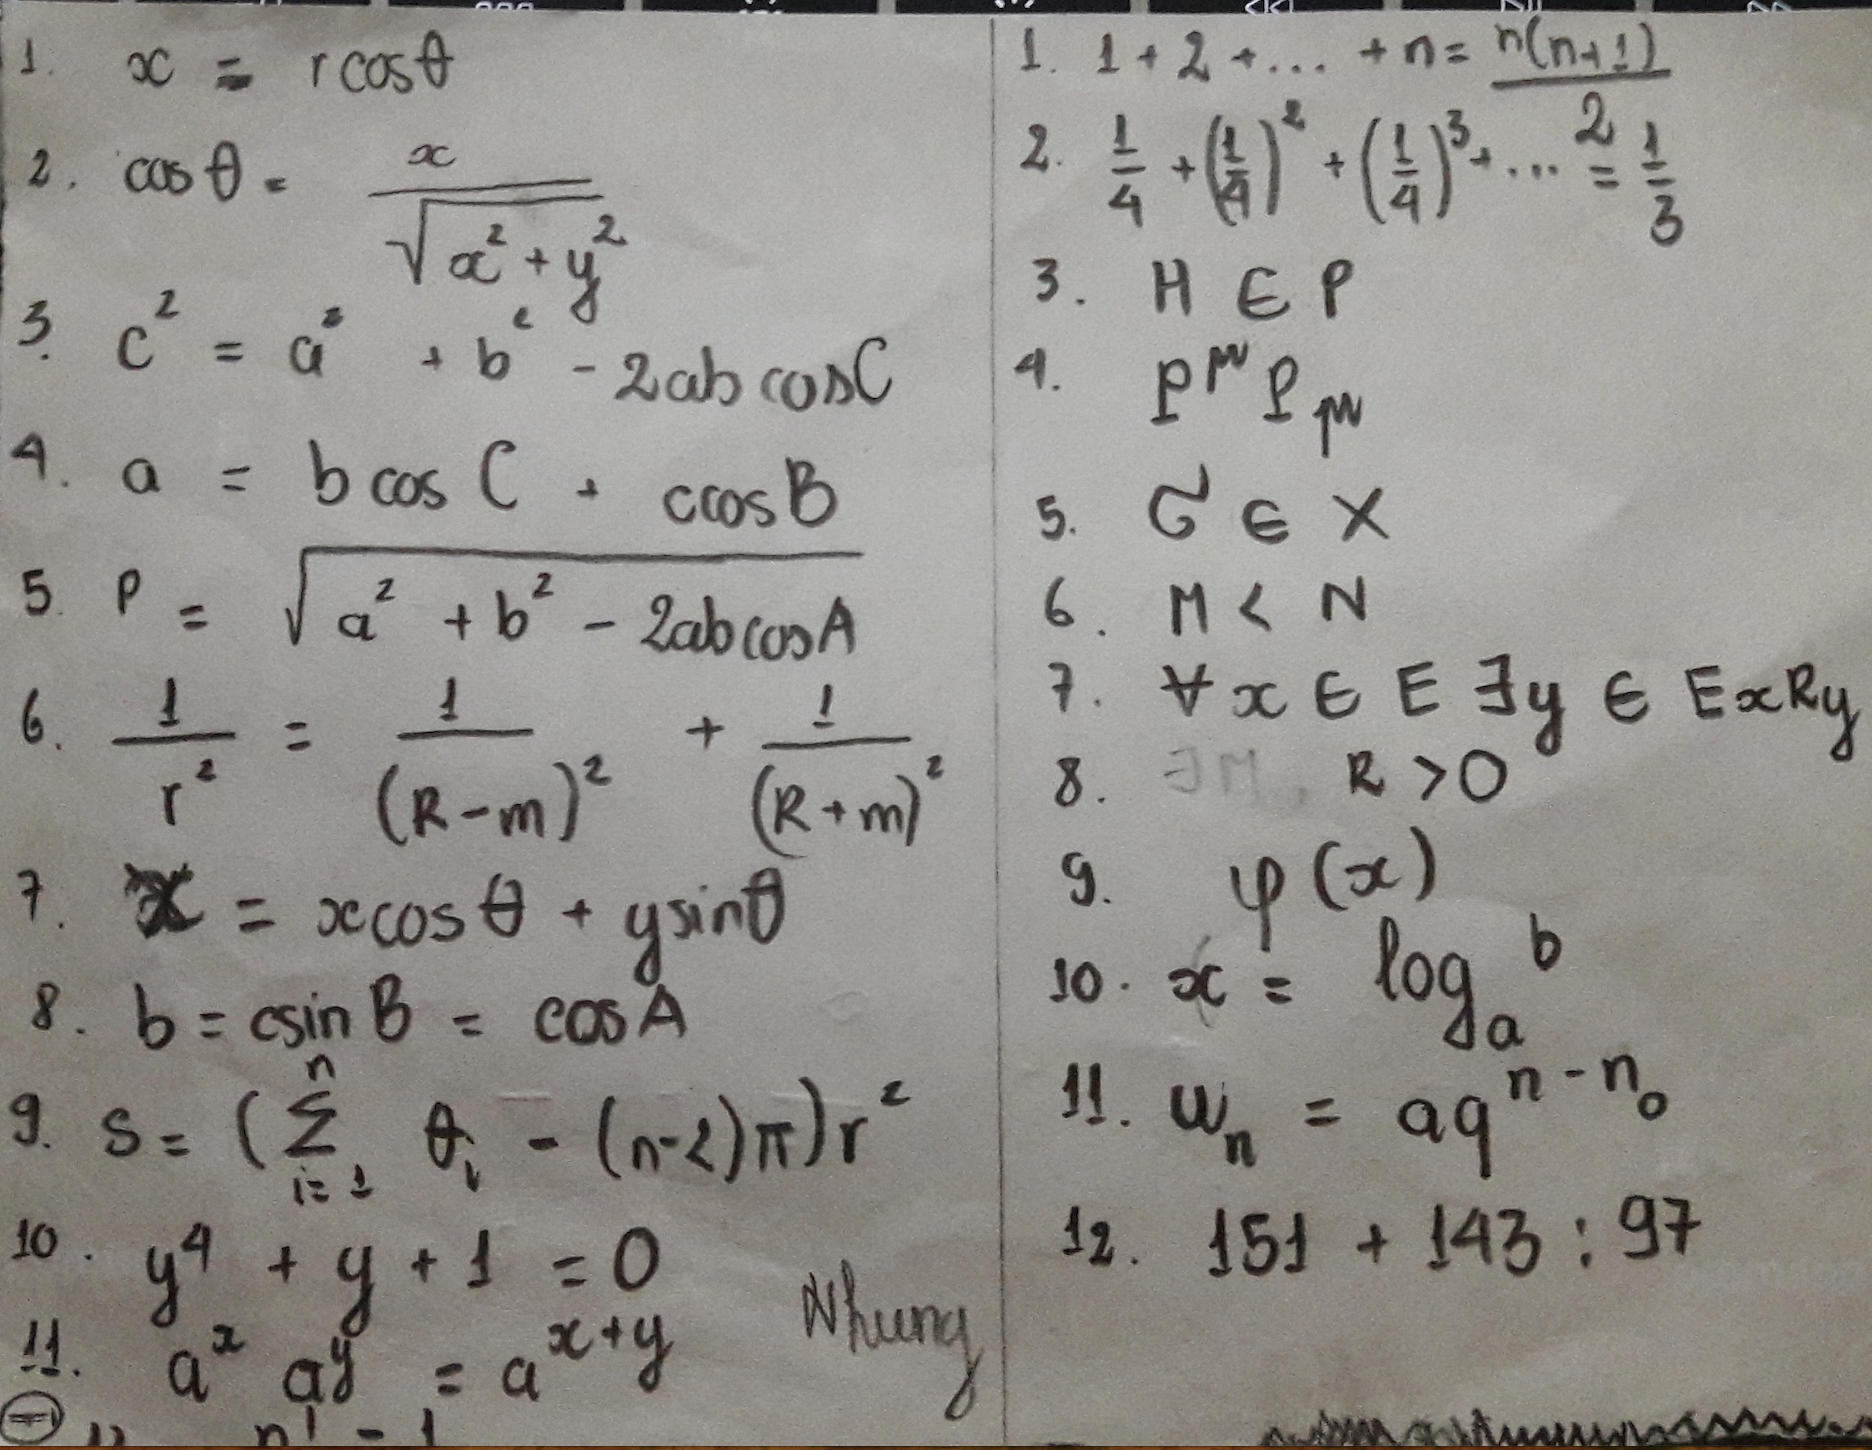
\includegraphics[width=0.45\linewidth]{Exp_sample1}
			\vspace{0.5cm}
			\caption{Ví dụ một biểu thức mẫu.}
		\end{figure}
	\end{frame}
	
	\begin{frame}{Xây dựng tập ảnh biểu thức}
		\begin{enumerate}
			\conti
			\item Tập hợp biểu mẫu đã cho viết, mang đi scan.
			\seti
		\end{enumerate}
		\begin{figure}[!h]
			\centering
			\includegraphics[width=0.85\linewidth]{Exp_sample}
			\vspace{0.2cm}
			\caption{Mẫu đã được điền và scan.}
		\end{figure}
	\end{frame}
	
	\begin{frame}{Xây dựng tập ảnh biểu thức}
		\begin{enumerate}
			\conti
			\item Sử dụng đoạn mã Matlab\footfullcite{qak} để tạo ảnh đầu vào quá trình huấn luyện.
			\seti
		\end{enumerate}
		\begin{center}
			\centering
			\includegraphics[width=0.45\linewidth]{EXP_2017_072_2A.png}
			\vspace{0.5cm}
			\captionof{figure}{Ví dụ một ảnh là input cho quá trình huấn luyện.}
		\end{center}
	\end{frame}
	
	\begin{frame}{Xây dựng tập ảnh biểu thức}
		\begin{enumerate}
			\conti
			\item Xây dựng bộ nhãn và vị trí bounding box của từng ký tự trong các ảnh đầu vào.
		\end{enumerate}
		\begin{center}
			\centering
			\includegraphics[width=0.5\linewidth]{tool}
			\vspace{0.5cm}
			\captionof{figure}{Giao diện công cụ hỗ trợ quá trình gán nhãn và xác định bounding box. }
		\end{center}
	\end{frame}
	
	\begin{frame}
		\begin{block}{Thông tin mô tả}
			\begin{itemize}
				\item Số người tham gia: khoảng 88 
				\item Số lượng ảnh:  2256. Trong đó có 1746 ảnh dùng cho training, 138 ảnh dùng cho quá trình validation và 372 ảnh để test.
				%				Trong đó, 372 ảnh test được thu thập từ 2 nguồn:
				%				\begin{itemize}
				%					\item[$-$] 192 ảnh được viết bởi người chưa từng tham gia viết cho quá trình thu thập ảnh huấn luyện.
				%					\item[$-$] 102 ảnh còn lại được viết bởi 15 người đã tham gia quá trình thu thập ảnh huấn luyện.
				%				\end{itemize}
				\item Số loại biểu thức: khoảng 552
				\item Số  người gán nhãn: 3
			\end{itemize}
		\end{block}
		\begin{center}
			\begin{tabular}{||c | c | c ||} 
				\hline
				Thông tin thêm & Tập huấn luyện & Tập kiểm tra\\[0.5ex] 
				\hline\hline
				\makecell{Tổng số ký tự} & 13697 & 2237 \\
				\hline
				\makecell{Chiều dài trung bình\\ của biểu thức} &$\approx{8}$  &$\approx{6}$\\
				\hline
				\makecell{Kích thước trung bình\\ của ký tự}& $24\times29$&$31\times41$\\
				\hline
			\end{tabular}
			\captionof{table}{Thông tin mô tả hai tập dữ liệu dùng cho huấn luyện và kiểm tra.}
		\end{center}
	\end{frame}
	%--------------------------------------------------
	\subsection{Đánh giá kết quả}
	\begin{frame}{Nhắc lại 4 phiên bản thử nghiệm}
		\begin{center}
			\begin{tabular}{||c | c | c | c | c||} 
				\hline
				Phiên bản & \makecell{  I } & \makecell{ II} & III &  \makecell{ IV}  \\ [0.5ex] 
				\hline\hline
				\makecell{Kích thước \\ảnh đầu vào}& 300x300 & 300x300 & 500x500 & 500x500 \\ 
				\hline
				\makecell{Kích thước \\default boxes\footnote{(max\_ratio, min\_ratio, min\_scale)}}& (20,90,0.1) & (8,50,0.03) & (8,50,0.03)& (8,50,0.03)\\ 
				\hline
				\makecell{Số lượng \\default boxes} & 8732 & 8732 & 24148 & 24024\\
				\hline
			\end{tabular}
			\captionof{table}{Sự khác nhau giữa 4 phiên bản thử nghiệm.}
		\end{center}
	\end{frame}
	
	\begin{frame}{Đánh giá định tính}
		\begin{center}
			\centering
			\includegraphics[width=0.775\linewidth]{compare_4.png}
			\vspace{0.5cm}
			\captionof{figure}{Kết quả nhận diện của 4 phiên bản thử nghiệm.}
		\end{center}
	\end{frame}
	\begin{frame}{Đánh giá định tính}
		\begin{center}
			\centering
			\includegraphics[width=0.775\linewidth]{compare_1.png}
			\vspace{0.5cm}
			\captionof{figure}{Kết quả nhận diện của 4 phiên bản thử nghiệm.}
		\end{center}
	\end{frame}
	\begin{frame}{Đánh giá định tính}
		\begin{center}
			\centering
			\includegraphics[width=0.85\linewidth]{compare_7.png}
			\vspace{0.5cm}
			\captionof{figure}{Kết quả nhận diện phiên bản IV trên ký tự nhỏ.}
		\end{center}
	\end{frame}
	
	\begin{frame}{Đánh giá định tính}
		\begin{center}
			\centering
			\includegraphics[width=0.95\linewidth]{result}
			\vspace{0.5cm}
			\captionof{figure}{Một số ảnh kết quả sau quá trình nhận dạng của phiên bản IV.}
		\end{center}
	\end{frame}
	
	\begin{frame}{Đánh giá định lượng}
		\begin{itemize}
			\item Điều kiện đánh giá
			\begin{itemize}
				\item [$-$] Cùng tập ảnh test gồm 372 ảnh.
				\item [$-$] Chỉ số đánh giá: $mAP$.
				\item [$-$] Máy chạy đánh giá: Ubuntu 14.04 LTS, Intel Core i5- 2500M 3.30GHz, 8GB RAM.
			\end{itemize}
			\item Kết quả
			\begin{center}
				\begin{tabular}{||c | c | c | c | c||} 
					\hline
					phiên bản & I&II&III&IV\\[0.5ex] 
					\hline\hline
					mAP&$\approx$0.58&$\approx$0.51&$\approx$0.64&$\approx$0.65\\
					\hline
					\makecell{Số lượng ký tự\\ nhận dạng được}&1581&1054&1837&1920\\
					\hline
					\makecell{Số file ảnh\\ không xử lý được}&4/372&8/372&0/372&0/372\\
					\hline
				\end{tabular}
				\captionof{table}{Kết quả mAP của 4 phiên bản thử nghiệm.}
			\end{center}
		\end{itemize}
	\end{frame}
	
	\begin{frame}{Kết quả}
		\begin{center}
			\centering
			\includegraphics[width=0.775\linewidth]{mAP.png}
			\vspace{0.5cm}
			\captionof{figure}{Trực quan kết quả mAP cho 4 phiên bản thử nghiệm.}
		\end{center}
	\end{frame}
	%--------------------------------------------------
	\section{Tổng kết}
	\subsection{Ưu điểm}
	\begin{frame}{Ưu điểm}
		\begin{itemize}
			\item Hệ thống có thể nhận diện được ký tự ở nhiều kích thước khác nhau.
			\item Nhận diện được nhiều biểu thức mà nếu chỉ dùng kỹ thuật phân vùng thì khó có thể làm được (ví dụ như biểu thức có ký tự dính nhau).
			\item Nhận diện được nhiều loại ký tự.
		\end{itemize}
	\end{frame}
	\subsection{Nhược điểm}
	\begin{frame}{Nhược điểm}
		\begin{itemize}
			\item Khi có nhiều ký tự trong ảnh thì hệ thống nhận diện gặp nhiều khó khăn.
			\item Tốc độ xử lý một ảnh còn chậm.
			\item Bộ phân tích cú pháp đơn giản.
			\item Các ký tự hoàn toàn trùng lên nhau dễ bị bỏ sót (dấu căn).
		\end{itemize}
	\end{frame}
	
	\subsection{Hướng phát triển}
	\begin{frame}{Phát triển tập dữ liệu biểu thức}
		\begin{itemize}
			\item Sử dụng phiên bản IV để kiểm tra.
			\item Hai ảnh cụ thể trong 372 ảnh test không nhận được chỉ số dưới, cụ thể số 1.
		\end{itemize}
		\begin{center}
			\centering
			\includegraphics[width=0.6\linewidth]{M1E1}
			\vspace{0.5cm}
			\captionof{figure}{Trường hợp không nhận được chỉ số dưới.}
			\label{fig: m1}
		\end{center}
	\end{frame}
	\begin{frame}{Phát triển tập dữ liệu biểu thức}
		\begin{block}{Giải pháp}
			Bổ sung mẫu biểu thức chứa cụ thể $E\_1$ và $M\_1$ vào tập huấn luyện. Cụ thể, tăng cường 96 ảnh vào tập huấn luyện và 24 ảnh để test.
		\end{block}
		\begin{center}
			\centering
			\includegraphics[width=0.7\linewidth]{M1E1_res}
			\vspace{0.5cm}
			\captionof{figure}{ Kết quả nhận dạng sau khi được huấn luyện với dữ liệu bổ sung.}
		\end{center}
	\end{frame}
	
	\begin{frame}{Khắc phục lỗi nhận dạng sai ở ký tự lớn}
		\begin{block}{Giải pháp}
			Thu nhỏ nội dung ảnh.
		\end{block}
		\begin{center}
			\centering
			\includegraphics[width=0.775\linewidth]{ensmall.png}
			\vspace{0.5cm}
			\captionof{figure}{Ví dụ thu nhỏ ảnh.}
		\end{center}
	\end{frame}
	
	\begin{frame}{Khắc phục lỗi nhận dạng sai ở ký tự lớn}
		\begin{center}
			\centering
			\includegraphics[width=0.875\linewidth]{compare_future.png}
			\vspace{0.5cm}
			\captionof{figure}{Kết quả thu được sau khi thu nhỏ nội dung ảnh.}
		\end{center}
	\end{frame}
	
	\begin{frame}{Hướng phát triển khác}
		\begin{itemize}
			\item Những điều cần kiểm tra:
			\begin{itemize}
				\item [$-$]Ảnh chứa đựng các ký tự nghiêng.
				\item [$-$]Ảnh có nhiễu.
				\item [$-$]Ảnh với nền khác màu trắng.
				\item [$-$]Ảnh chụp thay vì scan.
			\end{itemize}
			\item Những điều cần hoàn thiện:
			\begin{itemize}
				\item [$-$]Thêm phần hậu xử lý ở các giai đoạn nhận diện ký tự và sinh cây Lexed - BST.
				\item [$-$]Cải thiện khả năng nhận diện các ký tự có aspect ratio đặc biệt.
				\item [$-$]Tối ưu hoá bộ phân tích cú pháp. 
			\end{itemize}
		\end{itemize}
	\end{frame}
	\begin{frame}{Demo}
		\huge{Demo}
	\end{frame}
	\section*{Tham khảo}
	\begin{frame}
		\frametitle{Tham khảo}
		\printbibliography
	\end{frame}
	
	
	%------------------------------------------------
	\section*{Lời kết}
	\begin{frame}
		\Huge{\centering{Cảm ơn quý thầy cô và các bạn!}}
	\end{frame}
	
	\section*{Phụ lục}
	\begin{frame}{Phụ lục}
		\centering
		\colorbox{blue}{\textcolor{white}{\huge{Phụ lục}}}
	\end{frame}
	
	\begin{frame}{Công thức tính chỉ số mAP}
		Tính precision cho từng nhãn theo công thức\footfullcite{mAP}:
		\begin{align}
		precision = \frac{TP}{TP+FP},
		\end{align}
		\hspace{2cm}với $TP$ được viết tắt từ $True Positive$\footfullcite{mAP} và $FP$ từ $False Positive$\footfullcite{mAP}.\\
		Tính trọng số của từng nhãn trong tập dữ liệu kiểm tra theo công thức:
		\begin{align}
		class\_weight_i = \frac{N_i}{\sum_{u=0}^{106}N_u},
		\end{align}
		\hspace{2cm}với $N_i$ là số lượng ký tự thuộc nhãn $i$.\\
		mAP là trung bình có trọng số giữa $precision$ và $class\_weight$.
		
	\end{frame}
	\begin{frame}{Mẫu thu ký tự}
	\begin{center}
		\centering
		\includegraphics[width=0.75\linewidth]{data_sample.jpg}
		\vspace{0.5cm}
		\captionof{figure}{Ví dụ một mẫu thu ký tự đã được viết.}
	\end{center}
\end{frame}
	
	\begin{frame}{Cấu trúc mạng VGG16}
		\begin{center}
			\centering
			\includegraphics[width=0.95\linewidth]{vgg16.png}
			\vspace{0.5cm}
			\captionof{figure}{Cấu trúc mạng VGG16}
		\end{center}
	\end{frame}
	
	\begin{frame}{Những lỗi sai của hệ thống nhận dạng}
		\begin{center}
			\centering
			\includegraphics[width=0.775\linewidth]{phuluc_loi}
			\vspace{0.5cm}
			\captionof{figure}{Trường hợp sinh chuỗi Latex sai khi biểu thức chứa các ký tự có chân.}
		\end{center}
	\end{frame}
	
	\begin{frame}{Những lỗi sai của hệ thống nhận dạng}
		\begin{center}
			\centering
			\includegraphics[width=0.775\linewidth]{phuluc_sainhan}
			\vspace{0.5cm}
			\captionof{figure}{Trường hợp hệ thống gán sai nhãn cho những ký tự có nét tương tự nhau.}
		\end{center}
	\end{frame}
	%----------------------------------------------------------------------------------------
	
		%--------------------------------------------------
	%----------SUBSUB: LOSS----------------------
	%--------------------------------------------------
	\subsubsection{Mục tiêu huấn luyện}
	
	\begin{frame}
		\frametitle{Mục tiêu huấn luyện - "Hệ quy chiếu" ?}
		\begin{center}
			\centering
			\includegraphics[width=0.6\linewidth]{LOSSSS.png}
			\captionof{figure}{Độ lệch về kích thước}
		\end{center}
	\end{frame}
	\begin{frame}
		\frametitle{Mục tiêu huấn luyện - "Hệ quy chiếu" ?}
		\begin{center}
			\centering
			\includegraphics[width=0.6\linewidth]{LOSSX.png}
			\vspace{0.3cm}
			\captionof{figure}{Độ lệch về vị trí trọng tâm}
		\end{center}
	\end{frame}
	
	\begin{frame}
		\frametitle{Mục tiêu huấn luyện}
		\begin{block}{Mục tiêu huấn luyện}
			\begin{itemize}
				\item Cực tiểu chênh lệch về vị trí.
				\item Cực đại độ tin cậy của nhãn.
			\end{itemize}
		\end{block}
		
	\end{frame}
	
	
\end{document}